\chapter{Teorie}
\label{2-Teorie}

\section{OpenStreetMap}
\label{OpenStreetMap}

\subsection{Vznik}
\label{vznik}
OpenStreetMap (OSM) je projekt, jež vznikl s cílem vytvoření a sběru 
volně dostupných geografických dat a následně jejich možné vizualizace
do topografických map. Projekt založil Steve Coast v červenci roku 
2004 v Anglii. Jako inspirace mu posloužil projekt Wikipedia.

Zprvu projekt využívalo jen pár nadšenců, postupem času ale získal
projekt popularitu. S nárůstem počtu uživatelů se zvyšoval i objem dat.
Bylo tedy nutné navýšit kapacitu a zabezpečení serverů.
Také bylo potřeba zlepšit síťové řešení a infrastrukturu.
Tím je myšleno, že data byla rozdělena na více serverů.

V dubnu roku 2006 byla založena nadace OpenStreetMap Foundantion pro financováni 
projektu jako takového (zaměstnanců, běhu a zajištění bezpečnosti serverů atd.). \cite{wikiOSM}

\subsection{Struktura dat}
\label{struktura dat}
OSM data jsou nyní uložena v databázi PostgreSQL. \cite{OSMserver}

Pro samotnou výměnu dat ale slouží souborový formát {.osm}, který využívá datový
formát  XML. 
Jeho výhoda je jasná struktura, snadná orientace v kódu pro člověka. 
Nevýhodou je ovšem větší objem dat, který lze snížit kompresí. 

Prvky (elementy) jsou v OSM rozděleny na:
\begin{itemize}
    \item uzel (node) 
    \item cesta (way)
        \subitem neuzavřená
        \subitem uzavřená
        \subitem plocha (area)
    \item relace (relation) 
\end{itemize}

\subsubsection{uzel (node) }

Základním bodovým prvkem je uzel (node), který je definován jedinečným
identifikátorem ({\tt id=}). 
Je ukládána verze uzlu, časový údaj, kdy byl do databáze přidán
a je také uvedeno v jaké změně to bylo provedeno ({\tt changeset=~}).
Každý uzel má svoje souřadnice uloženy v souřadnicovém systému WGS~84 (EPGS 4326). 
Dále je možné připojit různé atributy (tag) tj. klíče s hodnotou ({\tt tag~k=~v=~}).
\\*
Příklad XML souboru pro uzel (strom):

{\scriptsize \begin{lstlisting}
<node id="2905214905" visible="true" version="1" changeset="22804106" 
      timestamp="2014-06-08T06:57:20Z" user="Salamandr" 
      uid="1708065" lat="50.1036981" lon="14.3897278">
    <tag k="natural" v="tree"/>
    <tag k="source" v="bing:ortofoto"/>
</node>
\end{lstlisting} }

\subsubsection{cesta (way) }

Označení pro liniový prvek je cesta (way), ta je vždy určena dvěma nebo více uzly.
Každá cesta má také svůj jedinečný identifikátor ({\tt way~id=~}) v rámci všech cest.
Má také základní atributy ({\tt id=*, visible=*, version=*, .. }), 
stejně jako u prvku uzel.
Dále však musí být seznam bodů, ze kterých se skládá.
Je zde uvedena pouze reference na id bodů, nikoliv jejich souřadnice.
Cestám lze taktéž přiřadit různé atributy.

Cesty se dále rozdělují na neuzavřené a uzavřené.
Jen uzavřené cesty mohou tvořit plošné objekty (area),
a jen těm se mohou přiřadit atributy určené pro plochy.
Například les ({\tt landuse=forest}).

Příklad XML souboru pro cestu:

{\scriptsize
\begin{lstlisting}
<way id="87249754" visible="true" version="2" changeset="34489106"
     timestamp="2015-10-07T11:52:41Z" user="Petr Dlouhý" uid="17615">
    <nd ref="1014526199"/>
    <nd ref="1014525941"/>
    <nd ref="1014526337"/>
    <nd ref="1014526022"/>
    <nd ref="1014526277"/>
    <nd ref="1014525984"/>
    <tag k="highway" v="path"/>
    <tag k="source" v="bing:ortofoto"/>
</way>
\end{lstlisting}
}
      
\subsubsection{relace (relation) }

Speciálním prvkem je relace (relation), do které lze zahrnout
jeden a více prvků. Mohou se do nich spojit prvky stejného druhu (uzel a uzel),
nebo různého (uzly, cesty nebo i relace).
Například dálnice je tvořena několika cestami (way), a ty
jsou zahrnuty do společné relace Dálnice D1. Nebo například turistická trasa
(od~KČT) může být relace sdružující, jak liniové prvky
(cesty, pěšiny), tak i bodové (rozcestníky, vyhlídky, apod. ).

U atributů popsaných na OpenStreetMap Wikipedii \cite{OSMfeatures} je vždy uvedeno
k jakému druhu prvku je
vhodné, či nevhodné je použít (dle komunity uživatelů OSM). Pokud se stane, že je použit
na~jiný, než doporučený druh prvku, může být následně problém v některých vykreslovačích. Viz \ref{Vykreslovače}
\begin{figure}[hbt]%[p]
    \centering
    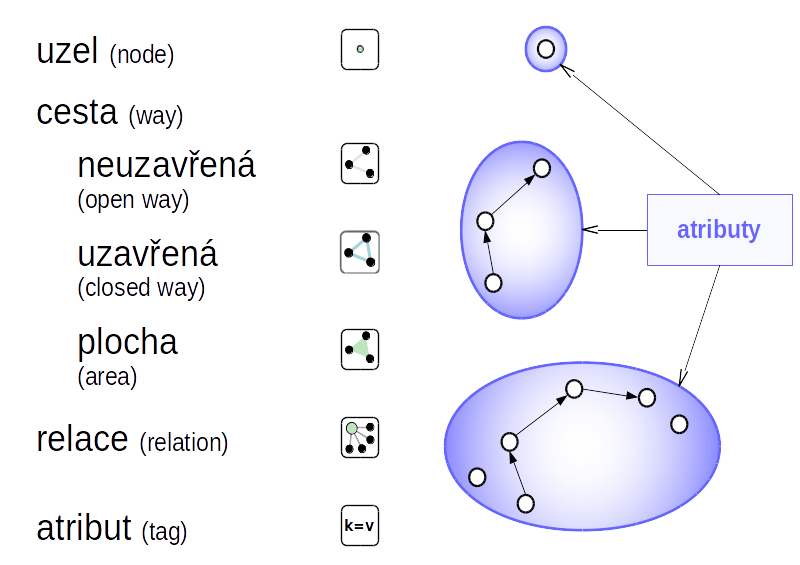
\includegraphics[scale=0.6]{./pictures/OSMelements.png}
    \caption{Rozdělení prvků OSM, vlastní tvorba}
    \label{fig:rozdělení OSM prvků}
\end{figure}


\subsection{Změna licence}
\label{změna licence}

Původně byla data OSM a generované grafické dlaždice distribuovány pod licencí
Creative~Commons~AllributionShare~Alike 2.0 (CC~BY~SA~2.0).

Tato licence umožňovala užití (distribuci ale i editaci) díla (dat) pod podmínkou,
že bude uveden zdroj OpenStreetMap.org ve viditelné části
vytvořených mapových dlaždic \cite{OSMlicence}.

  \begin{figure}[hbt]
    \centering
      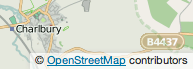
\includegraphics[scale=0.75]{./pictures/attribution_example.png}
      \caption{Příklad umístění licence,
                zdroj \url{http://www.openstreetmap.org/copyright}}
      \label{fig:attribution_example}
  \end{figure} 

V roce 2012 byla licence publikovaných dat změněna na Open Data Commons
Open Database Licence (ODbL).
Důvodem byla lepší licenční ochrana dat v databázi. 
Starší licence (CC BY-SA) chránila data pouze pomocí autorského zákona. 
Sice obě licence jsou "Uveďte autora" a "Zachovejte licenci", avšak rozdíl mezi
"starou" a "novou" je ten, že pokud někdo pod "starou" licencí (CC BY-SA),
vytvoří mapu (nebo jiné dílo) musí zachovat stejnou licenci.
Nemusí však uvolnit přímo data, která při tom použil.

Data OSM pod novou licencí, je možné jakkoli upravit,
a zveřejnit pod jakoukoli novou licencí,
která je podobná s myšlenkou Opendata, 
za podmínky, že také uvolní všechny své doplňky a vylepšení.\cite{OSMlicenceChange}.

Tato změna licence přinesla problém
s~daty, které byly poskytnuty projektu za předchozí licence
(CC~BY~SA~2.0). Bylo nutné se dotázat každého z dřívějších
přispěvatelů dat, ať už právnických osob, tak i fyzických osob,
zdali souhlasí, že jejich data budou distribuována pod novou licencí.
U přispěvatelů, kteří k tomuto nesvolili, nebo ti co se nevyjádřili,
bylo nutné jejich příspěvky z~databáze OSM vymazat.
Tato situace nastala pouze ve zlomku případů (méně než 1 \%).
Nejvíce tato změna licencí ohrozila data v zemích jako je Polsko a Nový Zéland. \cite {OSMlicenceIssue}

V současnosti jsou tedy data OSM distribuována pod licencí ODbL a
generované grafické dlaždice pod licencí CC-BY SA 4.0. \cite{OSMlicence}

\subsection{Licence ODbL}
Licence ODbl \footnote{Plné znění (anglicky) viz na \url{http://opendatacommons.org/licenses/odbl/1.0/}}
se zabývá právní ochranou databází, včetně
veškerých autorských a příbuzných práv k databázi.

Licence ODbl umožňuje
\begin{itemize}
    \item    kopírovat, distribuovat a užívat data
    \item    vytvářet nová data z původních
    \item    měnit původní data
\end{itemize}

Při použití databáze s licencí ODbl, je
nutné připojit kopii přesného znění licence ODbl.
Při nakládnání s databází ponechat nedotčena veškerá autorská práva a
uvést její zdroj (nebo autora).
Veškeré odvozené databáze musí splňovat podmínky ODbl,
tj. buď přímo licence ODbl, nebo licence s ní kompatibilní.
\cite{Nesetril2013thesis}

\subsection{Zdroje dat}
\label{Zdroje dat}
Jak bylo zmíněno, byla snaha, aby mapová data tvořili jedinci prvotním
sběrem dat, tj. měřením vlastními GNSS (GPS, Glonass) přijímači a
znalostí místních poměrů (uzavřené silnice, stezky atd.).  A takto
vzniklé dílo volně užívat k vlastním potřebám. Komunita přispěvatelů se
zprvu pomalu, později poměrně rychle rozrostla a dnes čítá 3,7 milionů
registrovaných uživatelů s alespoň jednou vytvořenou změnou v OSM a
2,7 milionů účtů aktivních přispěvatelů.\cite{OSMstats}

Takto vzniklé mapové podklady byly velice vhodné i pro další projekt, dnes již
velice rozšířený a známý jako Geocashing (GC). Projekt GC začal mapové
podklady od OSM užívat a zároveň jeho uživatelé začali sami tvořit a
přispívat do OSM. 

Přispěvatelé dat do OSM musí respektovat licenci projektu OdbL.
Tudíž i jejich zdroj dat musí splňovat tuto licenci. Proto by měli
všechny svoje změny, které v OSM vytvoří, řádně ozdrojovat atributem
s~klíčem 
{\tt source}.
V případě vlastního sběru dat se vyplňuje hodnotou
{\tt source=survey} ,
popřípadě uvést zdroj, odkud čerpali. Pokud tuto povinnost poruší a
použijí zdroj, jež není kompatibilní s licenční politikou OSM, tak ostatní 
přispěvatelé do~OSM tuto změnu, aby předešeli sporům, odstraní. 
V tomto případě dojde k odstranění celé sady změn, byť by v~ní byl pouze jeden prvek, jenž to poruší.

Druhým významným zdrojem dat jsou soukromé subjekty (společnosti).
Většinou jde o podkladové zdroje dat, například ortofoto, které jsou
vhodné pro obkreslování silničních síti z~leteckých nebo
satelitních snímků. V~jejich případě to
bylo řešeno písemným svolením, nebo smlouvou. Významným zdrojem
podkladových map pro obkreslování byly mapy vyhledávače Bing od společnosti
Microsoft. Ta svolila použít jejich letecké snímky většiny
obydlené pevniny. \footnote{\url{http://wiki.openstreetmap.org/wiki/Bing}}

Třetím zdrojem dat a zároveň postupně dominujícím, co do jeho obsahu, jsou
datové sady ze státního sektoru. Tyto datové sady jsou nejvhodnějším zdrojem
dat.

\subsection{Importy}
\label{Importy}
Výraz import v tomto případě znamená začlenění většího množství dat z datové sady nebo datových sad
z~jednoho datového úložiště (databáze serveru) na jiný. Při velkých objemech dat
se využívá výkonu výpočetní techniky z důvodu její bezchybnosti, a také
z~důvodu časové náročnosti. Na člověku poté zbývá zvolit postup importu
a naprogramovat skript nebo program, podle něhož technika samotný proces
provede. 

Datové importy z veřejných databází do databáze OSM jsou velmi cenné. 
Otevřené geografické, ale i jiné, databáze státu a jeho veřejných institucí 
financovaných státem jsou komplexní. Komplexní v tom smyslu, že obsahují celistvý
soubor dat, protože je daná instituce vyžaduje ke svému chodu. Jistá nevýhoda tu 
ale může být, data nemusí být vždy úplně aktuální. Některá data mohou 
být sbírána a zveřejněna i s větším časovým odstupem.

V rámci České Republiky proběhlo již několik hromadných datových importů. Jak 
již bylo řečeno, více času zabere samotná příprava na import.
V~případě importu dat do OSM, nejen napsání skriptu, ale i nutná diskuze tohoto záměru
na~diskuzní konferenci Talk-cz. 

\subsection{Talk-cz}
\label{Talk-cz}
Tato diskuze probíhá přes posílání emailových zpráv do společné konference. 
Uživatelům chodí emaily z probíhající diskuze. Pokud na nějaký
chtějí reagovat, tak pošlou email na adresu serveru, na kterém diskuze
běží. Musí ale do předmětu zprávy (emailu) napsat Re: a předmět zprávy, na kterou reagují.
Server tyto zprávy pomocí 
předmětu a času řadí. Diskuze je poté k dispozici na webových stránkách.\footnote{\url{http://lists.openstreetmap.org/listinfo/talk-cz}}

\subsection{Vykreslovače}
\label{Vykreslovače}
Na hlavní stránce OSM (\url{http://www.openstreetmap.org}) je k dispozici mapová aplikace. Ta nabízí pět
„základních“ přednastavených vrstev vykreslených z~dat z OSM.
Pro snadné vykreslení dat do grafických dlaždic se používá takzvaný pseudo Mercatorovo
zobrazení nebo Web Mercator (EPSG 3857), a to proto, že snadno vykreslí celý povrch Země (až na velké zkreslení u pólů). 
První, kdo zobrazení Web Mercartor použil, byla spolčnost Google pro svoje mapy Google Maps.\cite{WebMercator}
%%% ML: mozna dodat screenshoty do prilohy?

\begin{itemize}
  \item Standardní vrstva - vykresluje všechny prvky přiměřeně.
  \item Cyklomapa - vykresluje cyklostezky, výškopis. 
  \item Dopravní mapa - vykresluje silniční a železniční sítě.
  \item MapQuest Open - podkladová mapa právě pro potřeby Geocaching.
  \item Humanitární mapa - vykresluje důležité veřejné služby a potlačuje ostatní prvky. 
\end{itemize}

Existují další stránky, jež kombinují data z OSM a jiných zdrojů a vytváří z nich tematické mapy.
Například mapu turistických a cyklistických tras vykresluje
pro celou Evropu mtbmap.\footnote{mtbmap.cz}

%%% priklad? mozna dodat hezky screenshot?
Zajímavými projekty jsou například ty, které k 2D mapě přidávají „třetí“ rozměr a
vytvářejí tzv. 2.5D mapu. Většinou jde o 3D zobrazení budov, mostů (dle
atributů), popřípadě i stromů.

%%% http://demo.f4map.com/#lat=50.1036063&lon=14.3898880&zoom=19


\section{Opendata}
\label{opendata}

Základní myšlenka otevřených dat vznikla v USA.
Ta říká, pokud vzniknou jakákoli data z veřejných peněz, měla by tedy být
veřejně přístupná. Některé studie uvádí, že tento jev měl kladný efekt na ekonomiku.
\footnote{\url{http://www.worldbank.org/content/dam/Worldbank/document/Open-Data-for-Economic-Growth.pdf}}
\footnote{\url{http://www.otevrenadata.cz/res/data/001/003498.pdf}}

Proto jako první hlavní zdroj byly satelitní snímky povrchu Země (Landsat) %\footnote{\url{http://landsat.usgs.gov/}}
a digitální model terénu (projekt SRTM) %\footnote{\url{http://www2.jpl.nasa.gov/srtm/}}
s~rozlišením 30x30 m od NASA (pro pozdější vykreslení vrstevnic).

Tento trend se začal rozšiřovat zprvu do zemí západní Evropy
(Velké Británie, Francie či Německa), ale i země mimo Evropu.\cite{OpendataTrends}

V České republice se tomuto věnuje fond Otakara Motejla, založen na jeho počest,
a jeho hlavním projektem je Otevřená data. Spolupracuje s nadací Society Fund
Praha a Rekonstrukce Státu.
V rámci těchto uskupení je vyvíjen tlak na transparentnost veřejné správy,
zveřejňování smluv a dat státních institucí, jelikož jejich získání a údržba byla
placena z~veřejných zdrojů.
\\*
Otevřená data lze dělit na 5 stupňů,
dle otevřenosti.

\begin{figure}[hbt]%[p]
    \centering
    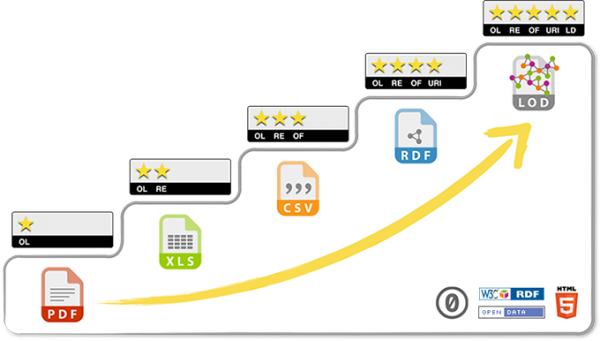
\includegraphics[width=0.8\textwidth]{./pictures/5star-steps.png}
    \caption{Stupně otevřenosti dat, převzato z \url{http://5stardata.info}}
    \label{fig:Stupně otevřenosti dat}
\end{figure}

\begin{itemize}

    \item   Data jsou dostupná v WWW stránek s jasnými licenčními
            podmínkami. Není zde žádný požadavek na datový formát,
            a proto není brán jako dostatečný způsob zveřejňování dat.
            Těmito daty ku příkladu jsou Webové Mapové Služby (WMS).
            Jsou veřejně k dispozici, avšak nezveřejňují přímo data,
            ale jen obrázky generované z nich.

    \item   Zveřejněná data jsou již ve strojově čitelném formátu,
            který je veřejně dobře znám. Nejčastěji se jedná
            o~charakter tabulky. Musí umožňovat přístup k~jednotlivým
            řádkům a obsahu buněk.

    \item   Třetí stupeň navíc od druhého vyžaduje, aby k~jeho čtení
            nebyl vyžadován speciální software, ale aby byl volně
            dostupný z WWW. Spadají sem tedy dokumenty formátů
            OpenOffice (Office Open XML, OpenDocument).
        \\* Pro~prostorová data například formáty GML, KML nebo
            GeoPackage.

    \item   U stupně otevřenosti 4 je v distribuované datové sadě
            povinnost zavést identifikaci entity ve tvaru
            Internationalized Resource Identifier (IRI)

    \item   U nejvyššího možného stupně otevřenosti je vyžadováno, aby
            distribuce splňovala standardy propojených dat (Linked
            Data).

\end{itemize}
%% http://opendata.gov.cz/standardy:stupne-otevrenosti

Díky této iniciativě došlo v rámci České Republiky ke zveřejnění
dat státních úřadů s různým úspěchem a stupněm otevřenosti.
Avšak tento trend zpřístupnění a zveřejňování pozvolna pokračuje.
Příkladem je Ministerstvo vnitra, Ministerstvo financí nebo Český úřad zeměměřický a katastrální.


\section{IPR Praha}
\label{IPR Praha}
IPR Praha je zkratka názvu prot Institut plánování a rozvoje
hlavního města Prahy. Tento institut se věnuje urbanismu, architektuře
a rozvoje města Prahy. Hlavním úkolem IPR je tvorba územního plánu
Prahy a významným úkolem IPR je zajišťovat zpracování geografických
informací. Spravuje data a mapy města Prahy. Od roku 2002 poskytuje
na~svých stránkách zdarma webové aplikace bez limitu využití.
Po~rozvoji Pražského geoportálu došlo k jejich většímu využívání.
Na~základě platných Pravidel pro poskytování dat a výstupů z~datových
souborů a datového skladu Geografického byly ode dne 1.~4.~2015
zveřejněny datové soubory a další webové služby. Tato data byla
uveřejněna pod licencí CC-BY SA 4.0 \cite{IPR}

\subsection{licence CC BY-SA 4.0}
\label{licence CC BY-SA 4.0}
Licence CC BY-SA 4.0 je zde uvedena ve zjednodušeném znění.

"Uživatel smí

\begin{itemize}
    \item   Sdílet - rozmnožovat a distribuovat materiál prostřednictvím jakéhokoli média v jakémkoli formátu
    \item   Upravovat - remixovat, změnit a vyjít z původního díla
\end{itemize}
pro jakýkoliv účel, a to i komerční.

Poskytovatel licence nemůže odvolat tato oprávnění do té doby, dokud dodržujete licenční podmínky.

Uveďte původ — Je Vaší povinností uvést autorství, poskytnout s dílem odkaz
na~licenci a vyznačit Vámi provedené změny. Toho můžete docílit jakýmkoli
rozumným způsobem, nicméně nikdy ne způsobem naznačujícím, že by poskytovatel
licence schvaloval nebo podporoval Vás nebo Váš způsob užití díla.

Zachovejte licenci — Pokud budete toto dílo upravovat, pozměňovat nebo
na~něj navazovat, musíte svoje odvozená díla vystavovat pod stejnou
licencí jako původní dílo."~\footnote{Citováno ze stánek CreativeCommons. \\*
Přesné znění licence viz na stránce https://creativecommons.org/licenses/by-sa/4.0/legalcode/}
